\documentclass[a4paper,fleqn]{cas-dc}

\usepackage[numbers,sort&compress]{natbib}
\usepackage{amsmath,amssymb,mathtools}
\usepackage{graphicx}
\usepackage{booktabs}
\usepackage{multirow}
\usepackage{tabularx}
\usepackage{siunitx}
\usepackage{lmodern}
\usepackage{microtype}
\usepackage{cleveref}
\usepackage{algorithm}
\usepackage{algorithmic}

\newtheorem{proposition}{Proposition}
\newdefinition{remark}{Remark}
\newproof{proof}{Proof}

\graphicspath{{figures/}}
\newcommand{\mgwo}{mGWO}
\newcommand{\mgwoa}{mGWO-a}
\newcommand{\acor}{ACO$_\mathbb{R}$}
\newcommand{\rehap}{REHAP}

\begin{document}
\let\WriteBookmarks\relax
\def\floatpagepagefraction{1}
\def\textpagefraction{.001}

\shorttitle{Benchmarking Metaheuristic-Tuned Nonlinear Controllers: Equal-Budget Validation, Digital Limits, and Generalization}
\shortauthors{J.~E.~Cervantes-Reyes et~al.}

\title [mode = title]{Pitfalls and Benchmarking of Metaheuristic-Tuned Nonlinear Controllers in Robotic Systems: Equal-Budget Validation, Digital Limits, and Generalization}

\author[1]{J.~E.~Cervantes-Reyes}[orcid=0009-0004-9457-3162]
\cormark[1]
\ead{cervantesreyesjesusedg16@gmail.com}
\credit{Conceptualization, Methodology, Software, Formal analysis, Investigation, Writing - original draft}

\author[1]{Ma.~de~los~Angeles~Alamilla~Daniel}
\ead{alamillameca@upp.edu.mx}
\credit{Supervision, Methodology, Writing - review \& editing}

\author[1]{Angel~Ricardo~Licona~Rodr{\'\i}guez}
\ead{arliconar@upp.edu.mx}
\credit{Conceptualization, Supervision, Project administration, Writing - review \& editing}

\affiliation[1]{organization={Universidad Polit\'ecnica de Pachuca},
            addressline={Carretera Pachuca-Cd. Sahag\'un km 20, Ex-Hacienda de Santa B\'arbara}, 
            city={Zempoala},
            postcode={43830}, 
            state={Hidalgo},
            country={Mexico}}

\cortext[1]{Corresponding author}

\begin{abstract}
Metaheuristics are widely used to tune nonlinear controllers for robotic manipulators and rehabilitation devices. However, prevailing benchmarking practices suffer from two critical flaws: evaluating the optimizer exclusively on the nominal plant model used for control design, and comparing algorithms under unequal computational budgets. Furthermore, tuned gains are rarely evaluated across unseen perturbed plants. We propose a rigorous validation protocol for \rehap{}, a two-degree-of-freedom lower-limb rehabilitation robot driven by backstepping control. The protocol trains each independent run on a distinct perturbed plant and evaluates performance across 20 unseen plants subjected to neuromuscular disturbance pulses. Under a strictly equal budget of 2000 cost evaluations (NFE) across 30 paired runs, a modified Grey Wolf Optimizer equipped with four escape mechanisms (\mgwo{}), canonical GWO, PSO, and \acor{} achieve statistically indistinguishable validation tracking quality (Friedman $p=0.65$, all Holm-adjusted pairwise $p\ge0.79$). Notably, PSO requires significantly more evaluations to attain its convergence plateau ($p=0.0014$). Mechanistic activation counters reveal that one escape mechanism in \mgwo{} never activates and its exploration parameter fails to reach zero within budget. A schedule-corrected variant (\mgwoa{}) restores benchmark precision on synthetic landscapes (Ackley median $0.108\to0.0094$) but provides no benefit for controller tuning, with \mgwo{} never outperforming canonical GWO. Crucially, nominal tuning drives gains toward the digital stability boundary ($49.6$~Hz oscillations at $100$~Hz sampling) and induces severe actuator saturation under perturbations. Our findings demonstrate that in low-dimensional controller tuning, proper budget-parameter alignment and digital limit enforcement matter far more than the ad-hoc addition of metaheuristic escape mechanisms.
\end{abstract}

\begin{highlights}
\item Equal-budget, paired statistical benchmark (NFE=2000, 30 runs) of GWO, mGWO, PSO, and ACO$_\mathbb{R}$.
\item Nominal plant tuning drives gains to the digital stability limit ($49.6$~Hz chatter at $100$~Hz sampling).
\item Gains tuned solely on the nominal model fail by $4$--$5$ orders of magnitude under parameter shifts.
\item Mechanistic ablation reveals hybrid escape mechanisms never activate or add no statistical advantage.
\item Demonstrates that hyperparameter-budget alignment outweighs algorithmic over-engineering in $D=4$.
\end{highlights}

\begin{keywords}
Rehabilitation robotics \sep Controller tuning \sep Robust control \sep Metaheuristics \sep Grey Wolf Optimizer \sep Statistical benchmarking
\end{keywords}

\maketitle

\section{Introduction}
Lower-limb rehabilitation robots must execute pre-planned therapeutic trajectories with high precision despite unpredictable patient-robot interactions and parameter uncertainties. Model-based nonlinear controllers such as backstepping \cite{krstic1995,khalil2002} exploit the Euler--Lagrange structure of manipulators \cite{spong2006}, and recent implementations often pair backstepping with disturbance estimation to mitigate parameter uncertainty \cite{peng2022,ren2025}. However, closed-loop tracking precision and transient stability heavily depend on selecting control gains. Because manual trial-and-error tuning is tedious, non-reproducible, and frequently sub-optimal, derivative-free metaheuristics have become the tool of choice \cite{azeez2023,dai2023}. Representative algorithms include the Grey Wolf Optimizer (GWO) \cite{mirjalili2014}, Particle Swarm Optimization (PSO) \cite{kennedy1995,shi1998,clerc2002}, and Continuous Ant Colony Optimization (\acor{}) \cite{socha2008,dorigo1997}. A proliferation of hybrid GWO variants have introduced multi-strategy initializations, Cauchy mutations, adaptive restarts, and local search routines to overcome premature convergence \cite{crepinsek2013,neri2012,blum2003}.

Despite hundreds of publications on metaheuristic-tuned controllers, two pervasive methodological flaws undermine the validity of comparative claims:
\begin{enumerate}
\item \emph{The nominal evaluation fallacy:} The optimizer searches for gains using the exact, unperturbed nominal plant model, and the tuned controller is then validated on that same nominal model \cite{sorensen2015,camacho2023}. The critical engineering question---whether the resulting gains remain stable and effective on plants that deviate from the design model---is routinely ignored.
\item \emph{Unequal computational budgets:} Algorithms are frequently compared across arbitrary iteration counts without standardizing the number of function evaluations (NFE), giving hybridized algorithms an unfair computational advantage \cite{kudela2022,kononova2014}.
\end{enumerate}

In robot-aided physical therapy, patient morphology (limb mass, segment inertia, muscle tone) varies substantially between individuals. Moreover, involuntary neuromuscular contractions such as spasticity, clonus, or tremors inject abrupt torque and position disturbances during rehabilitation exercises. Controllers tuned purely on nominal dynamics fail catastrophically under these physical conditions.

\paragraph{Contributions} This paper establishes a rigorous benchmarking methodology for metaheuristic-tuned nonlinear controllers, utilizing the \rehap{} two-degree-of-freedom lower-limb rehabilitation robot as a case study:
\begin{enumerate}
\item \emph{A robust validation protocol:} An optimization framework that trains on perturbed plants and independently validates tuned gains across 20 unseen plants under distinct neuromuscular pulse disturbance patterns (Sec.~\ref{sec:cost}).
\item \emph{Discovery and characterization of digital stability limits:} Analytical and numerical evidence showing that nominal tuning pushes control gains to the Nyquist limit of sampled-data zero-order-hold (ZOH) control ($49.6$~Hz oscillations at $100$~Hz sampling rate), inducing severe voltage saturation under real-world perturbations (Sec.~\ref{sec:results}A--B).
\item \emph{A strictly equal-budget, paired statistical benchmark:} A rigorous comparison of a modified GWO (\mgwo{}), schedule-corrected \mgwoa{}, canonical GWO, PSO, and \acor{} across 30 paired runs with Holm-adjusted Wilcoxon and Vargha--Delaney $A_{12}$ statistics (Sec.~\ref{sec:final}).
\item \emph{Mechanistic deconstruction of hybrid metaheuristic operators:} Empirical tracking of activation counters and ablation showing that complex escape mechanisms fail to activate or add no measurable benefit, formulating hypothesis $H^\ast$ on the primacy of hyperparameter-budget alignment over algorithmic over-engineering in low-dimensional controller tuning (Sec.~\ref{sec:mech}--\ref{sec:hyp}).
\end{enumerate}

\section{Related Work and State-of-the-Art Gap}
Backstepping provides a systematic Lyapunov design for strict-feedback systems \cite{krstic1995,khalil2002}. For fully actuated robotic manipulators, backstepping yields an inverse-dynamics control law with a filtered tracking error surface (Sec.~\ref{sec:control}). In controller tuning, metaheuristics balance exploration and exploitation \cite{crepinsek2013}. GWO achieves this balance through a linearly decaying control parameter $a$, PSO via inertia weights and stochastic acceleration coefficients, and \acor{} through a Gaussian mixture archive \cite{mirjalili2014,clerc2002,socha2008}. Hybrid and memetic extensions combine these population dynamics with local search operators \cite{neri2012,blum2003}.

The metaheuristics community has extensively critiqued metaphor-based algorithms \cite{sorensen2015,camacho2023} and benchmarks centered at the coordinate origin, which introduce structural search biases \cite{kononova2014,kudela2022}. Furthermore, implementation choices such as bound-handling mechanisms often dominate algorithmic behavior \cite{helwig2013}. Best practices dictate non-parametric hypothesis testing with family-wise error rate control (Holm correction \cite{holm1979}) and non-parametric effect sizes ($A_{12}$ \cite{vargha2000}) across identical evaluation budgets \cite{derrac2011}. In accordance with the No-Free-Lunch theorem \cite{wolpert1997}, no single optimizer should be expected to universally dominate across diverse objective landscapes.

Recent studies on metaheuristic-tuned nonlinear controllers for lower-limb exoskeletons \cite{faraj2023,zheng2026} and manipulators \cite{rezoug2022,azeez2023,dai2023} consistently tune and validate controllers on the nominal plant or on a single static uncertainty scenario, omitting equal-budget multi-algorithm comparisons. While scenario-based robust tuning has been explored for inverted pendulums \cite{zorlu2026}, it was restricted to a single PID family without multi-optimizer statistical benchmarking. Table~\ref{tab:sota} summarizes this critical gap in the recent literature.

\begin{table*}[t]
\caption{Metaheuristic-tuned nonlinear controllers for manipulators/exoskeletons: validation and comparison practices in recent literature.}
\label{tab:sota}
\begin{tabularx}{\textwidth}{@{}l p{3.2cm} p{2.8cm} X X@{}}
\toprule
Study & Application & Optimizer(s) & Train/validate on different plants & Equal-budget, multi-optimizer stats\\
\midrule
\cite{azeez2023} & 3-link flexible-joint manipulator & GA-tuned SMC & No (nominal only) & No (single optimizer)\\
\cite{dai2023} & Underwater vehicle-manipulator & GWO & No (nominal only) & No (single optimizer)\\
\cite{faraj2023} & Lower-limb rehab.\ exoskeleton & GWO & No (nominal only) & No (single optimizer)\\
\cite{zheng2026} & Lower-limb rehab.\ exoskeleton & GWO + fuzzy SMC & No (nominal only) & No (single optimizer)\\
\cite{rezoug2022} & Robotic manipulator & Extended GWO & No (nominal only) & No (single optimizer)\\
\cite{zorlu2026} & Cart-inverted pendulum & (FO)PID, scenario-tuned & Yes (uncertainty scenarios) & No (single optimizer family)\\
This work & \rehap{} lower-limb rehab.\ robot & \mgwo{}, GWO, PSO, \acor{} & Yes (20 unseen perturbed plants) & Yes (paired, equal NFE, Friedman/Holm/$A_{12}$)\\
\bottomrule
\end{tabularx}
\end{table*}

\section{System Dynamics and Backstepping Control}\label{sec:model}

\subsection{Euler--Lagrange robot dynamics}
\rehap{} is a mechatronic test bench developed for lower-limb physical therapy (hip and knee flexion/extension; see \cite{cervantes2025tesis,cervantes2025congreso}) with two revolute joints $q=[q_1,q_2]^\top$ driven by direct-drive DC servomotors ($r_i=1$). The rigid-body Euler--Lagrange dynamics with reflected motor inertia are
\begin{equation}
(M(q)+J_m)\ddot q + C(q,\dot q)\dot q + G(q) + F\dot q = \tau,
\label{eq:dyn}
\end{equation}
where $F=\mathrm{diag}(f_{v1},f_{v2})$, $J_m=\mathrm{diag}(J_{m1},J_{m2})$, and the elements of the symmetric inertia matrix $M(q)$ are $M_{11}=m_1l_{c1}^2+m_2(l_1^2+l_{c2}^2+2l_1l_{c2}\cos q_2)+I_1+I_2$, $M_{12}=M_{21}=m_2(l_{c2}^2+l_1l_{c2}\cos q_2)+I_2$, and $M_{22}=m_2l_{c2}^2+I_2$. With $h=m_2l_1l_{c2}\sin q_2$, the Coriolis matrix is
\begin{equation}
C(q,\dot q)=\begin{bmatrix}-h\dot q_2 & -h(\dot q_1+\dot q_2)\\ h\dot q_1 & 0\end{bmatrix},
\label{eq:coriolis}
\end{equation}
and the gravitational torque vector is
\begin{equation}
G(q)=\begin{bmatrix}(m_1l_{c1}+m_2l_1)g\cos q_1+m_2gl_{c2}\cos(q_1+q_2)\\ m_2gl_{c2}\cos(q_1+q_2)\end{bmatrix}.
\label{eq:gravity}
\end{equation}
For the nominal parameters listed in Table~\ref{tab:params}, $\det M(q)\ge2.4\times10^{-3}$ over $q_2\in[-\pi,\pi]$, ensuring that $M(q)$ remains uniformly positive definite. Moreover, $\dot M-2C$ is skew-symmetric, satisfying standard passivity properties \cite{spong2006}.

Neglecting armature inductance (as electrical time constants are substantially faster than rigid-body dynamics, $\tau_e \ll \tau_m$), the DC motor dynamics reduce to the algebraic torque-voltage relation:
\begin{equation}
\tau_i=\frac{K_a}{R_a}v_i-\frac{K_aK_b}{R_a}\dot q_i,\qquad |v_i|\le v_{\max}=24~\mathrm{V},
\label{eq:motor}
\end{equation}
which represents the physical actuation limit of the test bench ($\tau_{\max}=40$~N\,m is the nominal structural limit).

\begin{table*}[t]
\caption{Nominal parameters of the \rehap{} rehabilitation robot (SI units).}
\label{tab:params}
\begin{tabular*}{\tblwidth}{@{}LLLLLL@{}}
\toprule
Parameter & Value & Parameter & Value & Parameter & Value\\
\midrule
$m_1,m_2$ & 7.0, 1.0 kg & $l_1$ & 0.50 m & $l_{c1},l_{c2}$ & 0.186, 0.10 m\\
$I_1,I_2$ & $10^{-5}$, $4{\times}10^{-5}$ kg\,m$^2$ & $f_{v1},f_{v2}$ & 0.05 N\,m\,s/rad & $J_{m1},J_{m2}$ & 0.062 kg\,m$^2$\\
$K_a=K_b$ & 1.6206 N\,m/A & $R_a$ & 1.8 $\Omega$ & $v_{\max},\tau_{\max}$ & 24 V, 40 N\,m\\
\bottomrule
\end{tabular*}
\end{table*}

The therapeutic reference trajectory is a smooth quintic polynomial over $T=10$~s moving from $q_1=-\pi/2$ to $\pi/4$ and $q_2=0$ to $\pi/4$~rad, with zero initial and terminal velocities and accelerations. Numerical integration is performed using Runge--Kutta 4th order (RK4) with zero-order-hold digital control at $T_s=0.01$~s ($100$~Hz).

\subsection{Backstepping controller formulation}\label{sec:control}
Defining position tracking error $e=q-q_d$, gain matrices $K_1=\mathrm{diag}(k_{11},k_{12})$ and $K_2=\mathrm{diag}(k_{21},k_{22})$, virtual stabilizing control $\alpha=\dot q_d-K_1e$, and velocity error surface $z=\dot q-\alpha=\dot e+K_1e$, the commanded backstepping torque is synthesized as
\begin{equation}
\tau^c=M(q)(\ddot q_d-K_1\dot e-K_2z)+C(q,\dot q)\dot q+G(q)+F\dot q.
\label{eq:bs_tau}
\end{equation}
Motor armature voltages $v_i$ are computed by inverting~\eqref{eq:motor} while injecting $J_m\ddot q_r$ ($\ddot q_r=\ddot q_d-K_1\dot e$) to cancel reflected rotor inertia. Under nominal dynamics without saturation, the closed-loop error system satisfies
\begin{equation}
\dot z=-\Lambda(q)K_2z,\qquad \dot e=-K_1e+z,\qquad \Lambda=(M+J_m)^{-1}M.
\label{eq:errdyn}
\end{equation}
Because $\Lambda(q)$ is similar to a symmetric positive definite matrix, its eigenvalues are real and strictly contained in $(0,1)$. Along the prescribed trajectory, numerical evaluation yields $\lambda(\Lambda(q))\in[0.061, 0.908]$. The slow direction decays at roughly $6\%$ of the rate nominal $K_2$ suggests, explaining why optimizers tend to drive $k_{22}$ to large values.

\begin{proposition}[Nominal exponential stability, sufficient condition]\label{prop:stability}
For the nominal, continuous-time, unsaturated error dynamics~\eqref{eq:errdyn}, define, for each $q$ along the reference trajectory, $\lambda_2(q):=\lambda_{\min}\bigl(\tfrac12(\Lambda(q)K_2+K_2\Lambda(q)^\top)\bigr)$, the minimum eigenvalue of the symmetric part of $\Lambda(q)K_2$. If $\lambda_{\min}(K_1)>\tfrac12$ and $\inf_q\lambda_2(q)>\tfrac12$ along the trajectory, the origin $(e,z)=0$ is exponentially stable.
\end{proposition}
\begin{proof}
Consider the Lyapunov function candidate $V=\tfrac12\|e\|^2+\tfrac12\|z\|^2$. Taking the time derivative along trajectories of~\eqref{eq:errdyn} yields $\dot V=e^\top\dot e+z^\top\dot z=-e^\top K_1e+e^\top z-z^\top\Lambda K_2z$. Because quadratic forms depend solely on the symmetric part of their kernel matrix, $z^\top\Lambda K_2z\ge\lambda_2(q)\|z\|^2$ by the Rayleigh--Ritz theorem. Applying Cauchy--Schwarz and Young's inequality ($e^\top z\le\tfrac12\|e\|^2+\tfrac12\|z\|^2$),
\[
\dot V\le-\bigl(\lambda_{\min}(K_1)-\tfrac12\bigr)\|e\|^2-\bigl(\lambda_2(q)-\tfrac12\bigr)\|z\|^2\le-2cV,
\]
where $c=\min\{\lambda_{\min}(K_1)-\tfrac12,\ \inf_q\lambda_2(q)-\tfrac12\}>0$. Consequently, $V(t)\le V(0)e^{-2ct}$.
\end{proof}
\begin{remark}
Over the full operational workspace $q_2\in[-\pi,\pi]$, numerical evaluation confirms that for typical optimized gains (e.g., GWO run 19, $K_2=\mathrm{diag}(26.1, 78.4)$), $\lambda_2(q)\ge 4.41 > 0.5$ and $\lambda_{\min}(K_1)>0.5$ hold strictly across the workspace, guaranteeing continuous exponential stability. Conversely, near the lower search bound $lb=[1,1,1,1]$, $\inf_q\lambda_2(q)\approx0.061$, showing that while the sufficient condition fails for arbitrarily small gains, the optimizers reliably identify gains well inside the stable basin. Note that Proposition~\ref{prop:stability} assumes continuous-time, unsaturated operation; physical sampled-data and voltage saturation limits are governed by the digital limit analyzed in Sec.~\ref{sec:chatter}.
\end{remark}

The parameter vector to tune is $\theta=[k_{11},k_{12},k_{21},k_{22}]^\top\in\mathbb{R}^4$.

\section{Cost Function, Disturbance Model, and Validation Protocol}\label{sec:cost}

\subsection{Tracking objective and penalization}
For any candidate gain vector $\theta$, closed-loop dynamics are simulated for $T=10$~s. The scalar objective function is
\begin{equation}
\begin{aligned}
J(\theta)={}&\mathrm{RMS}_1+\mathrm{RMS}_2\\
&+\lambda_\tau\overline{\textstyle\sum_i\max(0,|\tau_i^c|-\tau_{\max})^2}+\lambda_{sat}f_{sat},
\end{aligned}
\label{eq:cost}
\end{equation}
where $\mathrm{RMS}_i=\sqrt{\frac{1}{K}\sum_{k=1}^K(q_i(t_k)-q_{di}(t_k))^2}$ denotes the true position root-mean-square tracking error, $\tau^c$ is the unconstrained commanded torque from~\eqref{eq:bs_tau}, the overbar denotes temporal averaging, $f_{sat}$ represents the fraction of time steps where motor voltage reaches saturation ($|v_i|>0.99v_{\max}$), and weights are fixed at $\lambda_\tau=1$ and $\lambda_{sat}=10$. Any simulation exhibiting numerical divergence or instability is assigned a penalty of $J=10^6$.

\subsection{Morphological uncertainty and neuromuscular pulses}
Parametric uncertainty is injected into all physical parameters $\vartheta_k\in\{m_1,m_2,l_{c1},l_{c2},I_1,I_2,f_{v1},f_{v2}\}$:
\begin{equation}
\tilde\vartheta_k=\vartheta_k(1+\rho u_k),\qquad u_k\sim\mathcal U(-1,1),\quad \rho=0.15,
\label{eq:uncertainty}
\end{equation}
representing inter-subject morphological variations ($\pm15\%$) encountered in clinical practice, while the controller retains the nominal parameters $\vartheta_k$.

In rehabilitation robotics, patients frequently exhibit spastic hypertonia, muscle spasms, or tremor. To model these abrupt joint torque/position disturbances, an external pulse train is added to measured feedback:
\begin{equation}
\begin{aligned}
q^m(t)&=q(t)+p(t),\\
p(t)&=\begin{cases}A & t\ge t_0,\ (t-t_0)\bmod P<w\\0&\text{otherwise},\end{cases}
\end{aligned}
\label{eq:pulse}
\end{equation}
with amplitude $A=0.01$~rad, period $P=2$~s, pulse width $w=0.05$~s, and onset $t_0=1$~s. In validation, an alternative, more aggressive spastic disturbance is also evaluated: $A=0.02$~rad, $P=2.5$~s, $w=0.1$~s, and $t_0=0.5$~s.

\subsection{Optimization problem and benchmarking protocol}\label{sec:probform}
Three tuning environments are defined: (A) nominal plant without pulses; (B) a single perturbed plant with disturbance pulses; (C) an ensemble mean cost over five fixed perturbed plants:
\begin{equation}
\bar J(\theta)=\tfrac15\textstyle\sum_{s=1001}^{1005}J(\theta;\mathrm{plant}_s).
\label{eq:barJ}
\end{equation}
The bounded optimization problem is
\begin{equation}
\theta^\star=\arg\min_{\theta\in[lb,ub]}J(\theta),\qquad lb=[1,1,1,1]^\top,
\label{eq:optprob}
\end{equation}
with $ub=[1000]^4$ in exploratory stages and $ub=[1000,1000,1000,600]^\top$ in the final protocol (justified in Sec.~\ref{sec:chatter}).

Because $J(\theta)$ contains non-differentiable kinks (voltage saturation, piecewise pulse disturbances) and severe step-penalty discontinuities ($10^6$) at the numerical stability boundary, gradient-based techniques fail to converge reliably. Derivative-free metaheuristics are budgeted strictly in terms of cost function evaluations (NFE). In the final confirmatory protocol, each independent run $k\in\{1,\dots,30\}$ trains all optimizers on the exact same perturbed training plant ($\text{seed}=3000+k$, paired design). Validation is performed by testing the resulting gains across 20 unseen perturbed plants (seeds 2001--2020) under both training and alternative disturbance patterns.

\section{Optimization Algorithms and Hyperparameters}\label{sec:opt}
All optimizers operate under a standardized budget of $NFE_{\max}=2000$. Table~\ref{tab:hyper} lists all hyperparameter values, kept invariant across all experiments.

\paragraph{Canonical GWO \cite{mirjalili2014}} A population of $N$ wolves is guided by the three best individuals ($X_\alpha, X_\beta, X_\delta$): $A_\ell=2ar_1-a$, $C_\ell=2r_2$, $X_\ell'=X_\ell-A_\ell\circ|C_\ell\circ X_\ell-X_i|$, with $r_1,r_2\sim\mathcal U(0,1)^D$, and updated position $X_i\leftarrow\mathrm{clip}((X_\alpha'+X_\beta'+X_\delta')/3)$. Parameter $a$ decays linearly: $a=2(1-t/T_{\max})$, where $T_{\max}=\lfloor(NFE_{\max}-N)/N\rfloor$. Elitism is enforced by archiving the overall best solution found.

\paragraph{Modified GWO (\mgwo{}) and Corrected \mgwoa{}} Built upon GWO, \mgwo{} integrates four hybrid mechanisms:
\begin{enumerate}
\item \emph{Informed seeding:} $n_s=5$ individuals are initialized from manual baseline gains $[5,5,4,4]$ and structured perturbations; the remaining $N-n_s$ are initialized uniformly.
\item \emph{Stagnation mutation:} A stagnation counter $c$ increments if leader cost does not improve by at least $\epsilon=10^{-6}$. When $c\ge c_{mut}=2$, the $n_{mut}=10$ worst individuals undergo Gaussian mutation ($\sigma=0.05(ub-lb)$).
\item \emph{Stagnation recovery:} If stagnation reaches $c\ge c_{res}=5$, a fraction $\phi=0.2$ of the worst population is re-initialized uniformly over $[lb,ub]$.
\item \emph{Elitist local search:} In every iteration, $n_{loc}=5$ candidates are sampled within a hypersphere of radius $r_{loc}=r_0(1-t/T_{\max})^\gamma$ around $X_\alpha$, replacing $X_\alpha$ only if superior.
\end{enumerate}
Crucially, mechanisms 2--4 consume additional function evaluations per iteration. In \mgwo{}, $T_{\max}$ is calculated assuming only population updates ($N$ evals/iter), causing the budget to exhaust before $t$ reaches $T_{\max}$, leaving parameter $a$ and local search radius $r_{loc}$ truncated at high exploration values. The corrected variant, \mgwoa{}, computes progress using actual evaluation consumption: $NFE/NFE_{\max}$. Algorithm~\ref{alg:mgwo} summarizes the execution flow.

\begin{algorithm}[t]
\caption{\mgwo{} (italicized text denotes added hybrid mechanisms)}
\label{alg:mgwo}
\begin{algorithmic}[1]
\REQUIRE $N, NFE_{\max}, [lb,ub], n_s, \epsilon, c_{mut}, c_{res}, \phi, n_{mut}, n_{loc}, r_0, \gamma$
\STATE \emph{Initialize $n_s$ agents from informed seeds; $N-n_s$ uniformly}
\STATE Evaluate all agents; $NFE\gets N$; $t\gets0$; $c\gets0$
\WHILE{$NFE < NFE_{\max}$}
\STATE Rank agents; set $X_\alpha, X_\beta, X_\delta$; $a\gets2(1-t/T_{\max})$
\FOR{each agent $i=1,\dots,N$}
\STATE $X_i\gets\mathrm{clip}\bigl((X_\alpha'+X_\beta'+X_\delta')/3\bigr)$
\ENDFOR
\STATE Evaluate updated agents; $NFE\gets NFE+N$
\STATE $c\gets0$ if $J(X_\alpha)$ improved by $\ge\epsilon$, else $c\gets c+1$
\IF{$c\ge c_{res}$}
\STATE \emph{Recovery: reinitialize worst $\phi N$ agents; $c\gets0$}
\ELSIF{$c\ge c_{mut}$}
\STATE \emph{Mutation: perturb worst $n_{mut}$ agents}
\ENDIF
\STATE \emph{Local search: sample $n_{loc}$ points around $X_\alpha$ at radius $r_{loc}$; replace $X_\alpha$ if improved}
\STATE $NFE\gets NFE+$ (extra evaluations); $t\gets t+1$
\ENDWHILE
\RETURN Best archived solution
\end{algorithmic}
\end{algorithm}

\paragraph{PSO \cite{kennedy1995,clerc2002}} Standard velocity update $v\leftarrow wv+c_1r_1\circ(p_i-x)+c_2r_2\circ(g-x)$, with inertia weight $w$ decaying linearly from $0.9$ to $0.4$, velocity clamping $|v|\le0.2(ub-lb)$, and reflection at bounds with velocity inversion.

\paragraph{\acor{} \cite{socha2008}} Continuous Ant Colony Optimization maintaining an archive of $k=50$ solutions. In each iteration, $m=5$ ants construct solutions via Gaussian mixture sampling centered on ranked archive solutions with selection weights $w_l$ and coordinate deviations proportional to average inter-solution distances.

\begin{table*}[t]
\caption{Hyperparameter configurations across all optimizers (strictly standardized).}
\label{tab:hyper}
\begin{tabular*}{\tblwidth}{@{}LL@{}}
\toprule
Algorithm & Parameters\\
\midrule
GWO & $N=20$\\
\mgwo{}, \mgwoa{} & $N=20, n_s=5, \epsilon=10^{-6}, c_{mut}=2, c_{res}=5, \phi=0.2, n_{mut}=10, \sigma=0.05, n_{loc}=5, r_0=0.1, \gamma=2$\\
PSO & $N=20, c_1=c_2=2.0, w_{\max}=0.9, w_{\min}=0.4, v_{\max}=0.2(ub-lb)$, reflection bounds\\
\acor{} & $k=50, m=5, q=0.1, \xi=0.85$\\
\bottomrule
\end{tabular*}
\end{table*}

\section{Experimental Results and Discussion}\label{sec:results}

\subsection{The nominal tuning fallacy}
Optimizing on the unperturbed nominal plant across 100--200 iterations leads all four algorithms to converge to virtually identical cost values ($J\approx4.24\times10^{-6}$ to $4.34\times10^{-6}$, differences $<1\%$). Because the backstepping controller encapsulates exact model parameters, arbitrarily large gains yield near-zero simulation errors. Consequently, the nominal plant is fundamentally incapable of discriminating optimizer efficacy.

\subsection{Identification of the digital stability limit}\label{sec:chatter}
Nominal tuning consistently pushes $k_{22}$ toward the upper bound ($k_{22}\approx900$). Fig.~\ref{fig:chatter} analyzes joint-2 tracking error as a function of $k_{22}$ and sampling step $T_s$. For $k_{22}\le700$, error remains perfectly smooth (peak-to-peak $<3.6\times10^{-8}$~rad). However, at $k_{22}\approx902$, high-frequency chatter erupts with a dominant spectral peak at exactly $49.6$~Hz---matching the Nyquist frequency of the $100$~Hz digital loop ($f_{Nyquist}=1/(2T_s)=50$~Hz). Halving the sampling period to $T_s=0.005$~s entirely eliminates this chatter, confirming that the instability is a zero-order-hold discretization artifact. At $k_{22}=1000$, the discrete loop becomes unstable. Thus, nominal optimization drives gains directly onto the digital stability boundary. To prevent discretization-induced instability, we enforce $ub(k_{22})=600$ in all subsequent protocols.

\begin{figure}[t]
\centering
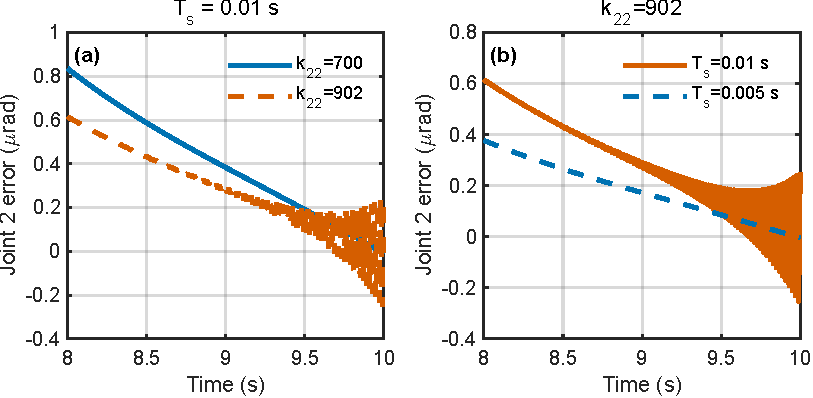
\includegraphics[width=\columnwidth]{articulo/fig_chatter.pdf}
\caption{Joint-2 tracking error in $[8,10]$~s under nominal plant simulation ($\mu$rad). (a) $T_s=0.01$~s: smooth tracking for $k_{22}\le700$, high-frequency chatter at $49.6$~Hz for $k_{22}\approx902$. (b) Halving $T_s$ to $0.005$~s suppresses the Nyquist oscillation, confirming a digital ZOH stability boundary.}
\label{fig:chatter}
\end{figure}

\subsection{Fragility of nominal gains under plant perturbations}\label{sec:fragility}
When gain sets tuned exclusively on the nominal plant are validated across 20 unseen perturbed plants with disturbance pulses, performance collapses catastrophically: validation cost median spikes to $1.3\times10^2$--$6.4\times10^3$, worst-case cost exceeds $10^6$, and motor voltages saturate during $7$--$79\%$ of the trajectory. In stark contrast, gains tuned under perturbed plants achieve validation costs of $\approx0.026$ (four to five orders of magnitude superior). Fig.~\ref{fig:loop} illustrates this mechanism: overly aggressive nominal gains amplify disturbance pulses, triggering severe voltage saturation and high-frequency limit cycles.

\begin{figure}[t]
\centering
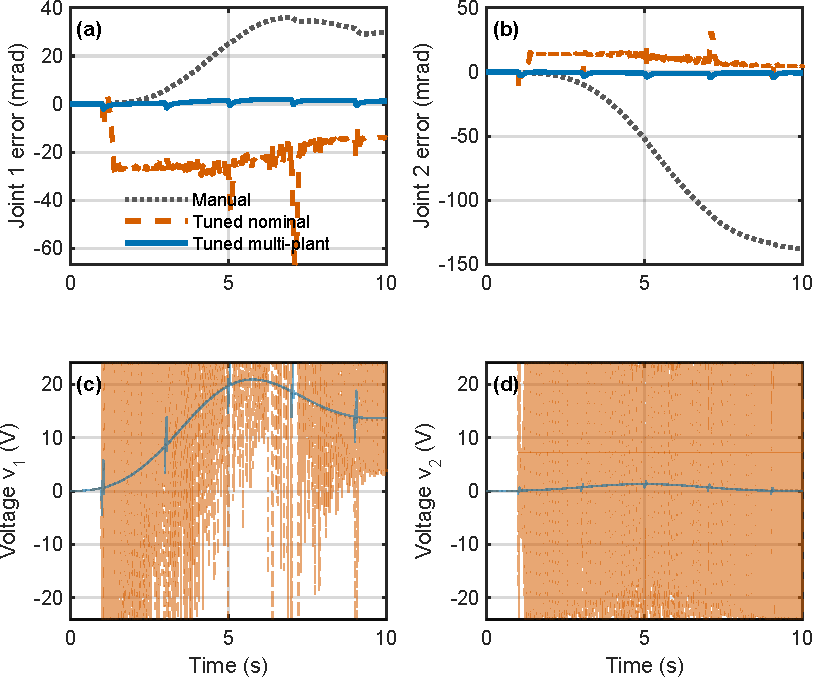
\includegraphics[width=\columnwidth]{articulo/fig_respuesta_lazo.pdf}
\caption{Closed-loop response on an unseen perturbed plant for manual, nominal-tuned, and multi-plant-tuned gains. (a,b) Tracking errors (mrad); (c,d) Armature voltages ($\pm24$~V limits). Nominal gains chatter between saturation boundaries; multi-plant gains maintain smooth tracking within $\approx10$~mrad without saturation.}
\label{fig:loop}
\end{figure}

\subsection{Confirmatory protocol: 30 paired runs}\label{sec:final}
Table~\ref{tab:final}(a) and Fig.~\ref{fig:finalval} present the results of the 30 paired runs under the final validation protocol ($NFE_{\max}=2000$).

\begin{table*}[t]
\caption{(a) Final validation protocol (30 paired runs, $NFE_{\max}=2000$): median validation cost on 20 unseen plants under training ($J_{val}$) and alternative ($J_{val}^{alt}$) disturbance pulses, interquartile range (IQR), worst-case cost, and evaluations to $5\%$ and $1\%$ convergence plateaus. (b) Generalization check on a cubic B\'ezier trajectory ($T=5$~s) without re-tuning.}
\label{tab:final}
\begin{tabular*}{\tblwidth}{@{}LLLLLLL@{}}
\multicolumn{7}{l}{\textbf{(a) Final Validation Protocol}}\\
\toprule
Algorithm & $J_{val}$ & IQR & $J_{val}^{alt}$ & Worst Case & $NFE_{5\%}$ & $NFE_{1\%}$\\
\midrule
\mgwo{}  & 0.02616 & 0.0040 & 0.0492 & 509 & 510  & 1398\\
\mgwoa{} & 0.02628 & 0.0030 & 0.0537 & 582 & 403  & 1183\\
GWO      & 0.02619 & 0.0017 & 0.0532 & 628 & 350  & 1220\\
PSO      & 0.02655 & 0.0039 & 0.0545 & 550 & 1320 & 1630\\
\acor{}  & 0.02603 & 0.0018 & 0.0448 & 577 & 645  & 1283\\
\bottomrule
\end{tabular*}
\vspace{1em}

\begin{tabular*}{\tblwidth}{@{}LLLLL@{}}
\multicolumn{5}{l}{\textbf{(b) Generalization Check on B\'ezier Trajectory}}\\
\toprule
Gain Configuration & RMSE $q_1$ (rad) & RMSE $q_2$ (rad) & ITSE ($\times10^{-5}$) & Voltage Saturation (\%)\\
\midrule
Manual $[5,5,4,4]$ & $2.35{\times}10^{-3}$ & $7.38{\times}10^{-3}$ & 4.98 & 0.00\\
\mgwo{} (run 2)    & $1.14{\times}10^{-4}$ & $9.36{\times}10^{-5}$ & 0.011 & 0.00\\
GWO (run 19)       & $1.30{\times}10^{-4}$ & $9.01{\times}10^{-5}$ & 0.015 & 0.00\\
\bottomrule
\end{tabular*}
\end{table*}

\begin{figure}[t]
\centering
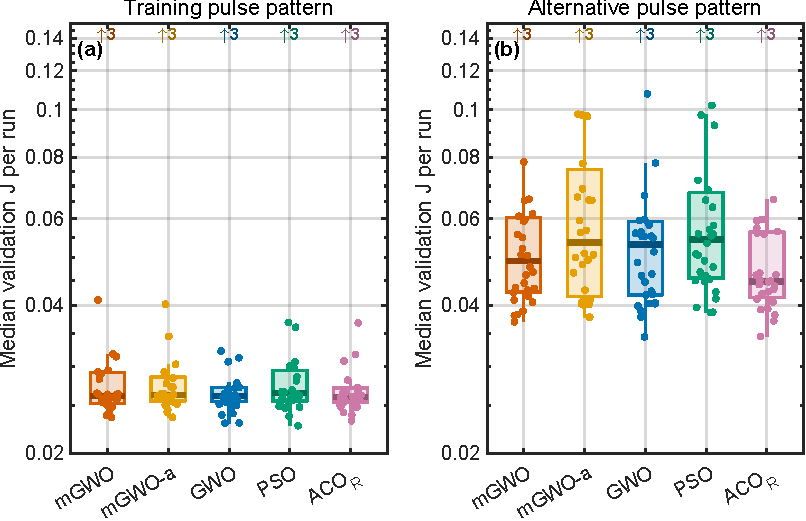
\includegraphics[width=\columnwidth]{articulo/fig_final_validacion.pdf}\\[4pt]
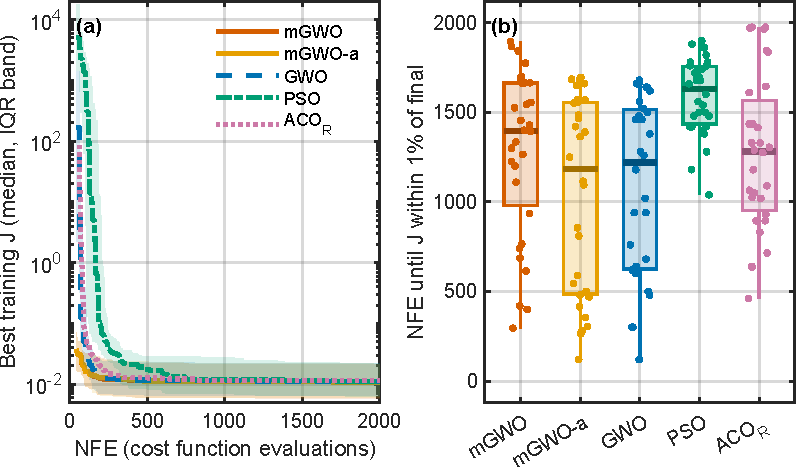
\includegraphics[width=\columnwidth]{articulo/fig_final_convergencia.pdf}
\caption{Confirmatory benchmarking over 30 paired runs (log scale). (a) Median validation cost under training disturbance pulses; (b) Validation cost under alternative pulses; (c) Convergence of best training cost vs.\ NFE (interquartile bands); (d) Evaluations required to reach within 1\% of final cost ($NFE_{1\%}$). All optimizers achieve indistinguishable validation quality; PSO converges significantly slower.}
\label{fig:finalval}
\end{figure}

\paragraph{Solution quality equivalence} Across all 30 paired runs, validation costs between the five optimizers are statistically indistinguishable (medians $0.02603$--$0.02655$, spread $<2\%$). The non-parametric Friedman test reveals no omnibus difference ($p=0.65$), and all pairwise Wilcoxon tests with Holm adjustment yield $p\ge0.79$, with Vargha--Delaney effect sizes concentrated at parity ($A_{12}\in[0.45, 0.55]$). Evaluating on the alternative pulse pattern confirms invariance ($p=0.24$). Schedule-corrected \mgwoa{} does not differ from baseline \mgwo{} ($p=1.0, A_{12}=0.46$).

\paragraph{Heavy-tail vulnerability} Every optimizer exhibits a heavy right tail in validation: 90th percentiles cluster at $0.70$--$0.72$, and worst-case costs reach $509$--$628$. This proves that optimizing average cost $\bar J$ fails to protect against extreme saturation events, which stem from plant uncertainty rather than optimizer deficiencies.

\paragraph{Convergence rate disparity} While asymptotic quality is identical, convergence speed differs significantly (Friedman $p=0.0014$ on $NFE_{1\%}$). As shown in Fig.~\ref{fig:finalval}(c)-(d), PSO requires substantially more evaluations ($1630$) than GWO ($1220$), \mgwo{} ($1398$), and \acor{} ($1283$) to reach its convergence plateau (Holm-adjusted $p$-values $0.001$--$0.042$).

\subsection{Benchmark landscapes and mechanistic deconstruction}\label{sec:scen}\label{sec:mech}\label{sec:hyp}
Table~\ref{tab:scen} details performance across synthetic landscapes (shifted Rastrigin and Ackley in $D=4$, with optima offset from the origin to eliminate center bias) and tight evaluation budgets ($300$ and $600$ NFE).

\begin{table*}[t]
\caption{Additional scenarios: median final cost (Holm-adjusted $p$-values vs.\ \mgwo{} in parentheses; bold indicates $p<0.05$).}
\label{tab:scen}
\begin{tabular*}{\tblwidth}{@{}LLLLL@{}}
\toprule
Algorithm & S1 (\rehap{}, 300 ev.) & S2 (\rehap{}, 600 ev.) & S3 (Shifted Rastrigin) & S4 (Shifted Ackley)\\
\midrule
\mgwo{}  & 0.0407 & 0.0402 & 2.98 & 0.108\\
\mgwoa{} & 0.0414 (0.35) & 0.0403 (0.47) & \textbf{2.00 (0.0095)} & \textbf{0.0094 ($3{\times}10^{-11}$)}\\
GWO      & 0.0407 (0.68) & 0.0394 (0.91) & 2.99 (0.60) & \textbf{0.0083 ($8.5{\times}10^{-9}$)}\\
PSO      & \textbf{0.0490 (0.017)} & \textbf{0.0420 (0.031)} & \textbf{1.17 ($1.9{\times}10^{-5}$)} & \textbf{$4.8{\times}10^{-4}$ ($3{\times}10^{-11}$)}\\
\acor{}  & 0.0443 (0.43) & 0.0370 (0.47) & \textbf{5.21 ($1.3{\times}10^{-5}$)} & \textbf{$2.1{\times}10^{-8}$ ($3{\times}10^{-11}$)}\\
\bottomrule
\end{tabular*}
\end{table*}

On shifted Ackley, canonical GWO significantly outperforms \mgwo{} ($0.0083$ vs.\ $0.108$, $p=8.5\times10^{-9}$). Activation counters explain this counterintuitive result: in \mgwo{}, local search consumed $18.5\%$ of all evaluations without finding improvements, and the stagnation recovery mechanism never triggered ($0$ activations across all runs because $c<c_{res}$). Furthermore, because $T_{\max}$ ignored the evaluation drain of local search, parameter $a$ terminated at $a\approx0.51$ instead of $0$, leaving residual exploration that crippled final convergence. Schedule-corrected \mgwoa{} fully restores benchmark precision ($0.108\to0.0094$), matching canonical GWO.

These findings support working hypothesis $H^\ast$: In low-dimensional controller tuning ($D=4$), hyperparameter-budget alignment and boundary handling exert far greater influence on tracking performance than the inclusion of complex escape mechanisms.

\section{Conclusions}\label{sec:concl}
This study presented a rigorous validation protocol and equal-budget statistical comparison for metaheuristic-tuned backstepping controllers on a lower-limb rehabilitation robot. The investigation establishes three key conclusions:
\begin{enumerate}
\item \emph{Nominal tuning is hazardous:} Optimizing on the nominal plant drives gains directly into the digital Nyquist boundary ($49.6$~Hz chatter at $100$~Hz sampling) and triggers catastrophic voltage saturation under model variations.
\item \emph{Algorithmic equivalence:} Under strictly equal evaluation budgets (2000 NFE across 30 paired runs), \mgwo{}, canonical GWO, PSO, and \acor{} achieve identical validation tracking quality (Friedman $p=0.65$), with PSO converging significantly slower ($p=0.0014$).
\item \emph{The fallacy of hybrid over-engineering:} Adding hybrid escape mechanisms to GWO failed to improve controller tuning and degraded precision on multimodal benchmarks due to internal parameter-budget mismatches.
\end{enumerate}

Future work will explore risk-sensitive objective functions such as Conditional Value-at-Risk (CVaR) to suppress validation heavy tails, derive analytical digital stability bounds for sampled backstepping, and deploy the validated gain sets onto the physical \rehap{} test bench.

\printcredits

\section*{Declaration of Competing Interest}
The authors declare that they have no known competing financial interests or personal relationships that could have appeared to influence the work reported in this paper.

\section*{Data and Code Availability}
The complete MATLAB simulation codebase, optimization routines, paired test data, and analysis scripts supporting this study are publicly available in our reproducible GitHub repository at: \url{https://github.com/UPP-Robotics/REHAP-Robust-Tuning}.

\printcredits

\bibliographystyle{cas-model2-names}
\bibliography{paper-refs}

\end{document}
